\PassOptionsToPackage{style=phys}{biblatex}
\documentclass{beamer}

%%%% PACKAGES

\usepackage{import}
\usepackage[toc,page]{appendix}
\usepackage[T1]{fontenc}
\usepackage[english]{babel}
\usepackage[utf8]{inputenc}
\usepackage{graphicx}
\usepackage{adjmulticol}
\usepackage[labelfont=bf]{caption}
\usepackage{float}
\usepackage{graphicx}
\usepackage{subcaption}
\usepackage{fancyhdr}
\usepackage{url}
\usepackage{amsmath} % collection de symboles mathématiques
\usepackage{amssymb} % collection de symboles mathématiques
\usepackage{amsthm}
\usepackage{bbm}
\usepackage{bm}
\usepackage{stmaryrd}
\usepackage{mathtools}
\usepackage{cancel}
\usepackage{titling}
\usepackage{nameref} % pour désigner des parties par leur nom
\usepackage{url} % pour mettre des URL
\usepackage{cite}
% \usepackage[sectionbib]{chapterbib}
% \usepackage{chapterbib}
\usepackage[numbers,sort&compress]{natbib}
% \usepackage[square,numbers,sectionbib]{natbib}
% \usepackage{bibunits}
% \usepackage{biblatex}
\usepackage{tabularx}
\usepackage{titlesec, blindtext, color}
% \usepackage{auto-pst-pdf}

%%%% TIKZ

\usepackage{pgf, tikz}
\usetikzlibrary{shapes.misc}
\usetikzlibrary{decorations.pathreplacing}

\tikzset{cross/.style={cross out, draw=black, minimum size=2*(#1-\pgflinewidth), inner sep=0pt, outer sep=0pt},
%default radius will be 1pt.
cross/.default={0.25pt},
    point/.style={
    thick,
    draw=black,
    cross out,
    inner sep=0pt,
    minimum width=4pt,
    minimum height=4pt,
    },
}

%%%% STYLE

\textheight=25 true cm
\textwidth= 20. true cm
\oddsidemargin=-1.75truecm
\evensidemargin=0.5truecm
\topmargin=-3 truecm

% \setlength{\topmargin}{-1cm}
% \setlength{\headheight}{0.43cm}
% \setlength{\headsep}{0.8cm}
% \setlength{\footskip}{0cm}
% \setlength{\textwidth}{17cm}
% \setlength{\textheight}{23.5cm}
% \setlength{\voffset}{-2.5cm}
% \setlength{\hoffset}{-0.25cm}
% \setlength{\oddsidemargin}{0cm}
% \setlength{\evensidemargin}{0cm}
\setlength{\parindent}{0pt}
\setlength{\footskip}{1.5cm}

\setlength{\droptitle}{-1cm}

\setcounter{tocdepth}{3}
\setcounter{secnumdepth}{3}

\definecolor{lcolor}{rgb}{0,0,0.6} % définition de la couleur des liens pdf
\usepackage{hyperref}
\hypersetup{pdftex,colorlinks=true,
linkcolor=lcolor,
citecolor=lcolor,
urlcolor=lcolor,
hyperindex=true,
hyperfigures=false} % fichiers pdf 'intelligents', avec des liens entre les références, etc.

\definecolor{gray75}{gray}{0.75}

\AtBeginDocument{\addtocontents{toc}{\protect\thispagestyle{empty}}}

% \titleformat{\chapter}[hang]{\vspace{-50pt}\huge\bfseries}{\thechapter\hspace{20pt}\textcolor{gray75}{|}\hspace{20pt}}{0pt}{\huge\bfseries}
\titleformat{\subsection}[block]{\hspace{0em}}{\large\textbf\thesubsection}{1em}{\large\textbf}
\titleformat{\subsubsection}[block]{\hspace{0em}}{\Small\textbf\thesubsubsection}{1em}{\Small\textbf}

\usepackage{etoolbox}
\makeatletter
\patchcmd{\@chap@pppage}{\thispagestyle{plain}}{\thispagestyle{empty}}{}{}
\makeatother

\captionsetup{font=normalsize}
\captionsetup[sub]{font=scriptsize}

%%%% COMMANDS

\providecommand{\ie}{\textit{i.e.}~}

%\renewcommand*\thesection{\arabic{section}}

\makeatletter
\providecommand*\bigcdot{\mathpalette\bigcdot@{.5}}
\providecommand*\bigcdot@[2]{\mathbin{\vcenter{\hbox{\scalebox{#2}{$\m@th#1\bullet$}}}}}
\makeatother

\providecommand{\appropto}{\mathrel{\vcenter{
  \offinterlineskip\halign{\hfil$##$\cr
    \propto\cr\noalign{\kern2pt}\sim\cr\noalign{\kern-2pt}}}}}

\providecommand\encircle[1]{%
  \tikz[baseline=(X.base)]
    \node (X) [draw, shape=circle, inner sep=0] {\strut #1};}

\providecommand\phantomarrow[2]{%
  \setbox0=\hbox{$\displaystyle #1\to$}%
  \hbox to \wd0{%
    $#2\mapstochar
     \cleaders\hbox{$\mkern-1mu\relbar\mkern-3mu$}\hfill
     \mkern-7mu\rightarrow$}%
  \,}

\providecommand{\myparagraph}[1]{\paragraph{#1}\mbox{}\\\vspace{-5pt}}

\providecommand{\isEquivTo}[1]{\underset{#1}{\sim}}

\makeatletter
\providecommand{\subalign}[1]{%
  \vcenter{%
    \Let@ \restore@math@cr \default@tag
    \baselineskip\fontdimen10 \scriptfont\tw@
    \advance\baselineskip\fontdimen12 \scriptfont\tw@
    \lineskip\thr@@\fontdimen8 \scriptfont\thr@@
    \lineskiplimit\lineskip
    \ialign{\hfil$\m@th\scriptstyle##$&$\m@th\scriptstyle{}##$\crcr
      #1\crcr
    }%
  }
}
\makeatother

% \makeatletter
% % Original \l@section:
% %\renewcommand*\l@section{\vskip 6pt plus 1pt minus 1pt
% %                         \@dottedtocline{1}{1.5em}{2.3em}}
% % Modified \l@section:
% \renewcommand*\l@section{\ifnum\c@tocdepth>\z@\vskip 6pt plus 1pt minus 1pt \fi
%                          \@dottedtocline{1}{1.5em}{2.3em}}
% \makeatother

\providecommand\smallO[1]{
      \mathchoice
         {% mode \displaystyle
            \ensuremath{\mathop{}\mathopen{}{\scriptstyle\mathcal{O}}\mathopen{}\left(#1\right)}
         }
         {% mode \textstyle
            \ensuremath{\mathop{}\mathopen{}{\scriptstyle\mathcal{O}}\mathopen{}\left(#1\right)}
         }
         {% mode \scriptstyle
            \ensuremath{\mathop{}\mathopen{}{\scriptscriptstyle\mathcal{O}}\mathopen{}\left(#1\right)}
         }
         {% mode \scriptscriptstyle
            \ensuremath{\mathop{}\mathopen{}{o}\mathopen{}\left(#1\right)}
         }
   }

%%%% PATCH

% \makeatletter
% \let\orig@document\document
% \let\orig@enddocument\enddocument
% \def\sa@document{%
%   \endgroup
%   \global\let\enddocument\sa@enddocument
%   \sa@atbegindocument
% }
% \def\sa@enddocument{%
%   \sa@atenddocument
%   \global\let\document\orig@document
%   \global\let\enddocument\orig@enddocument
%   \begingroup
%   \@ignoretrue
%   \def\@currenvir{document}%
%   \aftergroup\endinput
% }
% \makeatother

\usepackage[mode=buildnew,subpreambles=true]{standalone}
\usepackage{cancel}
\usepackage{calc}

%%%%% BEAMER TEMPLATE

\makeatletter
\let\insertsupervisor\relax
\renewcommand\supervisortitle{in collaboration with}
\mode<all>
{
  \renewcommand\supervisor[1]{\def\insertsupervisor{#1}}
  \titlegraphic{}
}
\makeatother

\AtEveryCitekey{\clearfield{title}}
\setbeamercolor{bibliography entry author}{fg = black}
\ExecuteBibliographyOptions{doi=false}

%%%%% MACROS

\renewcommand{\FigureFrom}[2]{
  [{\usebeamercolor[fg]{caption source} from:} \fullcite{#1}\ifblank{#2}{}{ (Fig.~#2)}]
}

% https://tex.stackexchange.com/questions/199218
\usetikzlibrary{arrows,shapes}
\newcommand{\tikzmark}[2]{\tikz[baseline,remember picture]{\node[anchor=base] (#1){#2};}}

%%%%% CUSTOM COLOURS

% colorblind accessible palette ("red", "green", "blue", "yellow") contrasting with pink (#E85E8A)
% https://davidmathlogic.com/colorblind/#%23000000-%23E85E8A-%23CC78BC-%23D55E00-%230173B2-%23ECE133
\definecolor{red}{HTML}{CC78BC} % purple (#CC78BC)
\definecolor{green}{HTML}{029E73} % orange (#D55E00)
\definecolor{blue}{HTML}{0173B2} % blue (#0173B2)
\definecolor{yellow}{HTML}{ECE133} % yellow (#ECE133)

%%%%% INFORMATION

\title{Collective motion in large deviations of active particles}
\shorttitle{Large deviations of active particles (\href{https://doi.org/10.1103/PhysRevE.103.022603}{PRE \textbf{103}, 022603 (2021)})}

\author{Yann-Edwin Keta}

\location{DAMTP StatPhys \& SoftMat seminars}

\supervisor{E. Fodor, F. van Wijland, M.E. Cates, and R.L. Jack}

\date{02/03/2021}

%%%%% DOCUMENT

\begin{document}

%% TITLE PAGE

{
\setbeamertemplate{footline}{}
\makeatletter
    \setbeamertemplate{headline}[default]
    \def\beamer@entrycode{\vspace*{-\headheight}}
\begin{frame}[noframenumbering]

\vspace*{-4mm}
{
 \hspace*{-\beamerleftmargin}%
\begin{minipage}{\paperwidth}
\includegraphics[width=\paperwidth]{header.eps}
\end{minipage}
}

\titlepage

\vspace{-20pt}
\begin{center}
{\href{https://doi.org/10.1103/PhysRevE.103.022603}{Phys. Rev. E \textbf{103}, 022603 (2021)}}\\
\href{https://github.com/yketa/DAMTP_MSC_2019_Wiki}{\footnotesize \faGithub~ yketa/DAMTP\_MSC\_2019\_Wiki}
\end{center}

\hfill
\begin{minipage}{0.5\linewidth}
\centering
\includegraphics[height=0.75cm]{cambridge.eps}
\end{minipage}
\hfill
\begin{minipage}{0.42\linewidth}
\centering

\includegraphics[height=0.75cm]{uparis.eps}
\end{minipage}
\hfill

\end{frame}
}

%% TABLE OF CONTENTS

{\footerwithoutframenumber
\begin{frame}<beamer>[noframenumbering]{Contents}
  \tableofcontents
\end{frame}
}

%% PRESENTATION

\section{Active matter}

\subsection{Non-equilibrium systems}

\begin{frame}[t]{Non-equilibrium systems}

Non-equilibrium dynamics breaks time-reversal symmetry and thus detailed balance. \pause We can identify 3 general classes:
\begin{itemize}[<+->]
  \item Systems relaxing towards equilibrium.
  \item Systems with boundary conditions imposing steady currents.
  \item Active matter.
\end{itemize}

\only<2>{
\begin{example}
Thermal system adapting to its thermostat, glasses.
\end{example}
}
\only<3>{
\begin{example}
Sheared liquid, metal rod between two thermostats.
\end{example}
}
\only<4>{
\begin{definition}
System composed of self-driven units, \textit{active particles}, each capable of converting stored or ambient free energy into systematic movement.\footfullcitenomark{marchetti2013hydrodynamics}
\end{definition}
\begin{example}
Cell tissues, swarms of bacteria, schools of fish, flocks of birds.
\end{example}
}

\footfullcitenomark{berthier2019lectures}
\footfullcitenomark{cates2015motility}

\end{frame}

\begin{frame}{Non-equilibrium phenomenon in active matter: swarming (Vicsek)}

% \begin{itemize}
%   \item[$\rightarrow$] Aligning self-propelled disks with repulsive interactions (Vicsek model).
% \end{itemize}
%
% \begin{equation}
% \dot{\boldsymbol{r}}_i = v_0 \begin{pmatrix} \cos \theta_i \\ \sin \theta_i \end{pmatrix} - \mu \nabla_i U(\{\boldsymbol{r}_j\}),~ \dot{\theta}_i = \frac{1}{\tau} (\varphi_i - \theta_i) + \xi_i,~ \varphi_i = \arg(\dot{\boldsymbol{r}}_i)
% \end{equation}

\begin{minipage}{0.35\linewidth}
\begin{figure}
\centering
\includestandalone[width=\textwidth]{vicsek}
\end{figure}
\begin{equation}
\dot{\theta}_i = \frac{1}{\tau_p}(\varphi_i - \theta_i) + \xi_i
\end{equation}
\end{minipage}
\hfill
\begin{minipage}{0.6\linewidth}
\insertmovie{1}{vicsek.png}{vicsek.mp4}{}
\end{minipage}

\footfullcitenomark{vicsek1995novel}
\footfullcitenomark{szabo2006phase}

\end{frame}

\begin{frame}{Non-equilibrium phenomenon in active matter: MIPS}

% \begin{itemize}
%   \item[$\rightarrow$] Active Brownian particles with repulsive soft interactions.
% \end{itemize}
% \vspace{-5pt}
% \begin{equation}
% \dot{\boldsymbol{r}}_i = v_0 \begin{pmatrix} \cos \theta_i \\ \sin \theta_i \end{pmatrix} - \mu \nabla_i U(\{\boldsymbol{r}_j\}),~ \dot{\theta}_i = \sqrt{2 \tau^{-1}}\xi_i
% \end{equation}

\begin{minipage}{0.35\linewidth}
\begin{figure}
\centering
\includestandalone[width=0.75\textwidth]{abp}
\end{figure}
\begin{eqnarray}
\dot{\theta}_i = \sqrt{2 \tau_p^{-1}} \xi_i\\
\left<\boldsymbol{u}(\theta_i(0)) \cdot \boldsymbol{u}(\theta_i(t))\right> = e^{-t/\tau_p}
\end{eqnarray}
\end{minipage}
\hfill
\begin{minipage}{0.6\linewidth}
\insertmovie{1}{mips.png}{mips.mov}{}
\end{minipage}

\footfullcitenomark{cates2015motility}
\footfullcitenomark{keta2019cooperative}

\end{frame}

\subsection{Active Brownian particles}

\begin{frame}[t]{Active Brownian particles}

% \begin{itemize}
%   \item[$\rightarrow$] \only<1>{$N$}\only<2->{$\color{red}N$} active Brownian particles (ABPs).
% \end{itemize}
\begin{eqnarray}
&\dot{\boldsymbol{r}}_i = - \only<1>{\mu}\only<2-5>{\textcolor{red}{\mu}}\only<6->{\frac{1}{3}\textcolor{red}{\tilde{l}_{\rm p}^{-1}}} \nabla_i U(\{\boldsymbol{r}_j\}) + \only<1>{v_0}\only<2>{\textcolor{red}{v_0}} \boldsymbol{u}(\theta_i) + \sqrt{\only<1-4>{2 \only<1>{D}\only<2-4>{\textcolor{red}{D}}} \only<5->{\frac{2}{3}\textcolor{red}{\tilde{l}_{\rm p}^{-1}}} \vphantom{\frac{2}{3}\tilde{l}_{\rm p}^{-1}}} \boldsymbol{\eta}_i\\
&\dot{\theta}_i = \sqrt{2 \only<1>{D_r}\only<2-3>{\textcolor{red}{D_r}}\only<4->{\textcolor{red}{\tilde{l}_{\rm p}^{-1}}} \vphantom{\tilde{l}_{\rm p}^{-1}}} \xi_i
\end{eqnarray}
% \begin{itemize}
%   \item[$\rightarrow$] $U$ $\equiv$ WCA potential, $\boldsymbol{u}(\theta_i) \equiv (\cos\theta_i, \sin\theta_i)$, $\eta^{\alpha}_i$, $\xi_i$ $\equiv$ unit-variance zero-mean Gaussian white noises, \only<1-2>{$\only<2>{\color{red}}\sigma$ $\equiv$ diameter, }\only<1>{$\phi$}\only<2->{$\color{red}\phi$} $\equiv$ packing fraction.
% \end{itemize}

\only<2->{
\only<2>{7}\only<3-4>{5}\only<5>{4}\only<6->{3} control parameters: $\color{red} N$, $\color{red} \phi$, \only<2>{$\color{red} \sigma$, }\only<2-5>{$\color{red} \mu$, }\only<2>{$\color{red} v_0$, }\only<2-4>{$\color{red} D$, }$\color{red} \only<2-3>{D_r}\only<4->{\tilde{l}_{\rm p} = D_r^{-1}}\vphantom{\frac{l_p}{\sigma}}$.\\
\only<3->{
\begin{itemize}
  \item[$\rightarrow$] Units of space and time: $\sigma = 1$, $\sigma/v_0 = 1$.
  \only<5->{\item[$\rightarrow$] Stokes-Einstein relation: $D = \frac{1}{3}D_r = \frac{1}{3}\tilde{l}_{\rm p}^{-1}$.}
  \only<6->{\item[$\rightarrow$] Scaling of energy: $\mu = D$.}
\end{itemize}
}
}

\footfullcitenomark{nemoto2019optimizing}
\footfullcitenomark{redner2013structure}

\end{frame}

\begin{frame}{Active work}

\vspace{-15pt}
\begin{eqnarray}
\text{EOM}& \dot{\boldsymbol{r}}_i = \only<1-5>{v_0 \boldsymbol{u}(\theta_i) - D \nabla_i U + \sqrt{2 D} \boldsymbol{\eta}_i}\only<6->{{\color{red} v_0 \boldsymbol{u}(\theta_i)} {\color{green} - D \nabla_i U} + {\color{blue} \sqrt{2 D} \boldsymbol{\eta}_i}}\\ \pause
\text{dissipated power}& \dot{\mathcal{W}}_i = \sum_{i=1}^N \dot{\boldsymbol{r}}_i \circ \frac{1}{D} (\dot{\boldsymbol{r}}_i - \sqrt{2 D} \boldsymbol{\eta}_i)\\ \pause
& \frac{1}{\tau} \int_0^{\tau} \dot{\mathcal{W}}_i(t) \, \mathrm{d}t = \frac{N v_0^2}{D} \only<3-4>{w_{\tau}}\only<5->{{\color{CaPink} w_{\tau}}} + \only<3>{\frac{1}{\tau} [U(\tau) - U(0)]}\only<4->{\cancel{\frac{1}{\tau} [U(\tau) - U(0)]}}\\ \pause\pause
\text{active work}& {\color{CaPink} w_{\tau} = \frac{1}{v_0 N \tau} \sum_{i=1}^N \int_0^{\tau} \boldsymbol{u}(\theta_i) \circ \mathrm{d}\boldsymbol{r}_i} \\ \pause
& {\color{CaPink} w_{\tau}} = {\color{red} 1} + {\color{green} w_{f, \tau}} + \only<6>{{\color{blue} w_{\eta, \tau}}}\only<7->{\cancel{{\color{blue} w_{\eta, \tau}}}}
\end{eqnarray}
\pause

\pause
\hfill
\begin{minipage}{0.4\linewidth}
\centering
\bf Flocking
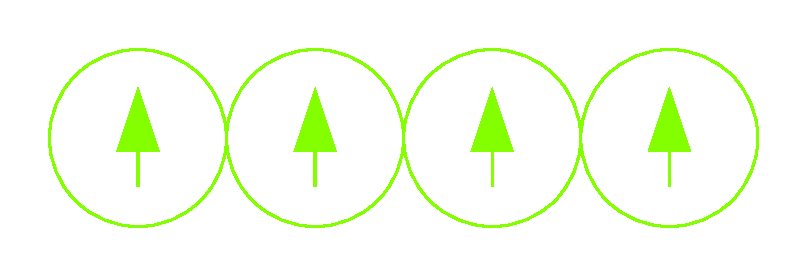
\includegraphics[width=\linewidth]{w1.eps}
$\boldsymbol{u}(\theta_i) \cdot \nabla_i U = 0 \Rightarrow \left<w_{\tau}\right> = 1$
\end{minipage}
\hfill
\begin{minipage}{0.4\linewidth}
\centering
\bf Jamming
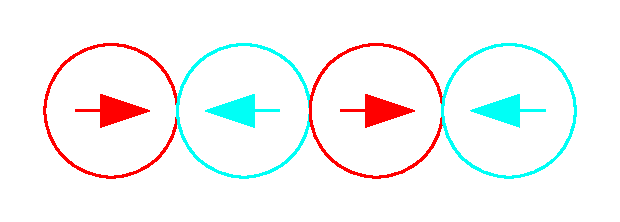
\includegraphics[width=\linewidth]{w0.eps}
$\dot{\boldsymbol{r}}_i = 0 \Rightarrow \left<w_{\tau}\right> = 0$
\end{minipage}
\hfill\hfill

\end{frame}

\section{Large deviation theory}

\subsection{Concepts and applications}

\begin{frame}[t]{Large deviation principle}

\footfullcitenomark{touchette2009large}

\begin{center}
$X_1, \ldots, X_n$ a sequence of (i.i.d.) random variables
\end{center}

\return
\begin{equation}
\left<X_i\right> = \mu,~ \left<(X_i - \mu)^2\right> = \sigma^2
\end{equation}

\return
\begin{equation}
\text{sample average}~ {\color{CaPink} R_n} = \frac{1}{n} \sum_{i=1}^n X_i
\end{equation}

\pause
\return

\only<2>{
\begin{center}
  \bf Law of large numbers
\end{center}
\begin{equation}
P\left(\lim_{n \to \infty} R_n = \mu\right) = 1
\end{equation}
}
\pause

\only<3>{
\begin{center}
  \bf Central limit theorem
\end{center}
\begin{equation}
P(R_n) \underset{n \to \infty}{\sim} \mathcal{N}\left(\mu, \frac{\sigma^2}{n}\right)
\end{equation}
}
\pause

\only<4>{
\begin{center}
  \bf Large deviation principle
\end{center}
\begin{equation}
{\color{CaPink} R_n} \text{ satisfies a LDP } \Leftrightarrow -\log P({\color{CaPink} R_n} = r) \underset{n \to \infty}{\sim} n {\color{blue} I}(r)
\end{equation}
\begin{equation}
{\color{blue} I} \equiv \text{ rate function of } {\color{CaPink} R_n} \Leftrightarrow P({\color{CaPink} R_n} = r) \asymp \exp(- n {\color{blue} I}(r))
\end{equation}
}

\end{frame}

% \begin{frame}{LDP example: sample mean of Gaussian random variables}
%
% \begin{center}
% $X_1, \ldots, X_n$ independent random variables with Gaussian distribution $(\mu, \sigma)$
% \end{center}
%
% \return
% \begin{equation}
% \text{sample average}~ {\color{CaPink} R_n} = \frac{1}{n} \sum_{i=1}^N X_i
% \end{equation}
%
% \pause
% \return
% \begin{equation}
% P({\color{CaPink} R_n = r}) = \sqrt{\frac{n}{2 \pi \sigma^2}} e^{-n(r - \mu)^2/(2\sigma^2)} \only<3->{\asymp \exp\left(-n {\color{blue} (r - \mu)^2/(2\sigma^2)}\right)}
% \end{equation}
%
% \pause
% \return
% \begin{equation}
% \lim_{n \rightarrow \infty} - \frac{1}{n} \log P({\color{CaPink} R_n} = r) = {\color{blue} (r - \mu)^2/(2\sigma^2) = I(r)}
% \end{equation}
% % \begin{itemize}
% % \item[$\Rightarrow$] $R_n$ satisfies a large deviation principle.
% % \end{itemize}
%
% \end{frame}

\begin{frame}[t]{LDP example: mean of random bits}

\begin{center}
$X_1, \ldots, X_n$ random bits, taking value $0$ or $1$ with equal probability
\end{center}

\begin{equation}
\text{sample average}~ {\color{CaPink} R_n} = \frac{1}{n} \sum_{i=1}^n X_i
\end{equation}

\pause
\return
\begin{equation}
\lim_{n \rightarrow \infty} - \frac{1}{n} \log P({\color{CaPink} R_n} = r) = {\color{blue} \log 2 + r \log r + (1 - r) \log(1 - r) = I(r)}
\end{equation}
\begin{equation}
P({\color{CaPink} R_n} = r) \asymp \exp(- n {\color{blue} I}(r))
\end{equation}

\only<3>{
\begin{figure}
\centering
\includegraphics[width=0.7\textwidth]{bits.eps}
\end{figure}
}

\only<4->{
\begin{figure}
\centering
\includegraphics[width=0.7\textwidth]{bits_CLT.eps}
\end{figure}

% \begin{itemize}
%   \item[$\rightarrow$] Deviations from the Gaussian fluctuations predicted by the Central Limit Theorem $\Rightarrow$ \textit{large} deviations.
% \end{itemize}
}

\end{frame}

\begin{frame}{Scaled cumulant generating functon}

\begin{equation}
\text{SCGF}~ {\color{green} \psi}(s) = \lim_{n \rightarrow \infty} \frac{1}{n} \log \left<\exp(-s n {\color{CaPink} R_n})\right>
\end{equation}

\pause
\return
\begin{center}
  \bf G\"artner-Ellis theorem
\end{center}
\begin{equation}
\begin{aligned}
{\color{green} \psi} \text{ is differentiable } \Rightarrow {\color{blue} I}(r) &= %\mathscr{L}_r({\color{green} \psi}) =
\sup_s \left\{- s r - {\color{green} \psi}(s)\right\} %\\ &= - s^*(r) r - {\color{green} \psi}(s^*(r))
\end{aligned}
\end{equation}
  % with $\mathscr{L}_r$ the Legendre transform with respect to $r$.

\footfullcitenomark{touchette2009large}

\end{frame}

\begin{frame}[t]{Analogy with equilibrium statistical mechanics: free energy}

\begin{center}
mean energy per particle for $n$ particles ${\color{CaPink} E_n}$
\end{center}

% \begin{center}
% $E_n \equiv$ energy of $n$ particles.
% \end{center}
\begin{equation}
\text{Boltzmann distribution}~ P_{\beta}(\omega) = \frac{e^{- \beta n {\color{CaPink} E_n(\omega)}}}{Z_n(\beta)}
\end{equation}

\pause
\return
\begin{equation}
\begin{aligned}
\text{SCGF}~ {\color{green} \psi_{\beta}}(\Delta\beta) &= \lim_{n \rightarrow \infty} \frac{1}{n} \log \int e^{- \Delta\beta n {\color{CaPink} E_n(\omega)}} P_{\beta}(\omega) \, \text{d}\omega\only<3->{\\
&= \lim_{n \rightarrow \infty} \frac{1}{n} \log \frac{Z_n(\beta + \Delta\beta)}{Z_n(\beta)}\\
&= \beta F(\beta) - (\beta + \Delta\beta) F(\beta + \Delta\beta)}
\end{aligned}
\end{equation}

\pause
\return
\begin{equation}
\text{free energy density}~ \beta F(\beta) = - \lim_{n \rightarrow \infty} \frac{1}{n} \log Z_n(\beta)
\end{equation}

\end{frame}

\begin{frame}{Analogy with equilibrium statistical mechanics: entropy}

\begin{equation}
{\color{green} \psi_{\beta}} \text{ is differentiable}\xRightarrow[\text{Gärtner-Ellis}]{} P_{\beta}({\color{CaPink} E_n}) \asymp \exp(-n {\color{blue} I_{\beta}}({\color{CaPink} E_n}))
\end{equation}

\pause
\return
\begin{equation}
P_{\beta}({\color{CaPink} E_n}) \asymp \exp(n(\underbrace{S({\color{CaPink} E_n})}_{\mathclap{\substack{\text{entropy}\\\equiv\text{number of states}}}} - \overbrace{\beta {\color{CaPink} E_n}}^{\mathclap{\substack{\text{Boltzmann}\\\text{function}}}} + \underbrace{\beta F(\beta)}_{\mathclap{\substack{\text{partition}\\\text{function}}}}))
\end{equation}

\pause
\return
\begin{equation}
{\color{blue} I_{\beta}}({\color{CaPink} E_n}) = -S({\color{CaPink} E_n}) + \beta {\color{CaPink} E_n} - \beta F(\beta)
\end{equation}

\pause
\return
\begin{equation}
{\color{blue} I_{\beta}}({\color{CaPink} E_n}) = 0 \Leftrightarrow F(\beta) = {\color{CaPink} E_n} - \frac{1}{\beta} S({\color{CaPink} E_n})
\end{equation}

\end{frame}

\begin{frame}{Application to trajectories: dynamical phase transitions}

\begin{center}
$d$-dimensional system of size $N$ represented by $\{\boldsymbol{X}_1(t), \ldots, \boldsymbol{X}_N(t)\}$
\end{center}

\begin{equation}
{\color{CaPink} R_{N \tau}} = \frac{1}{N \tau} \int_0^{\tau} \sum_{i=1}^N f(\boldsymbol{X}_i(t)) \, \text{d}t
\end{equation}
\pause
\begin{equation}
{\color{blue} I}(r) = \lim_{\tau \rightarrow \infty} -\frac{1}{N \tau} \log P({\color{CaPink} R_{N \tau}} = r),~ {\color{green} \psi}(s) = \lim_{\tau \rightarrow \infty} \frac{1}{N \tau} \log \left<e^{-s N \tau {\color{CaPink} R_{N \tau}}}\right>
\end{equation}

\pause
\return
\begin{table}
\begin{tabular}{c | c | c}
\rowcolor{CaLightPink}
\bf Quantity & \multicolumn{2}{c}{\bf Equilibrium counterpart}\\
\hline \hline
\rowcolor{white!90!CaLightPink}
$\{\boldsymbol{X}_i(t)\}$ & $\omega$ & Microstate in $(d+1)$-dim.\\
\rowcolor{white!80!CaLightPink}
${\color{CaPink} R_{N\tau}}$ & $E_n$ & Mean energy\\
\rowcolor{white!90!CaLightPink}
$s$ & $\Delta \beta$ & Inverse temperature\\
\rowcolor{white!80!CaLightPink}
${\color{green} \psi}$ & $\beta F(\beta) - (\beta + \Delta\beta) F(\beta + \Delta\beta)$ & Free energy\\
\rowcolor{white!90!CaLightPink}
${\color{blue} I}$ & $-S(E_n) + \beta E_n - \beta F(\beta)$ & Entropy
\end{tabular}
\end{table}

% \pause
% \return
% \begin{itemize}
%   \item[$\Rightarrow$] Singularities in $I_N/N$ and $\psi_N/N$ in the limit $\tau \rightarrow \infty$ and $N \rightarrow \infty$ $\Rightarrow$ \textit{dynamical phase transitions}.
% \end{itemize}

\end{frame}

\subsection{Biased trajectories and cloning algorithm}

\begin{frame}{Cloning algorithm}

\footfullcitenomark{jack2020ergodicity}
\footfullcitenomark{nemoto2016population}

\vspace{-20pt}
\begin{center}
equilibrium \textbf{canonical ensemble} $\to$ \textbf{biased ensemble} of trajectories
\end{center}
\begin{eqnarray}
% & {\color{green} \psi}(s) = \lim_{\tau \to \infty} \frac{1}{\tau} \log \int e^{-s \, N \, \tau \, {\color{CaPink} R_{N\tau}[\{\boldsymbol{X}_i(t)\}]}} P_{s = 0}[\{\boldsymbol{X}_i(t)\}] \, \mathscr{D}\{\boldsymbol{X}_i(t)\}\\
& P_s[\{\boldsymbol{X}_i(t)\}] \propto P_0[\{\boldsymbol{X}_i(t)\}] e^{-s N \tau {\color{CaPink} R_{N\tau}}}\\
& \left<\mathcal{A}\right>_s = \frac{\left<\mathcal{A} e^{-s \, N \, \tau \, {\color{CaPink} R_{N\tau}}}\right>}{\left<e^{-s \, N \, \tau \, {\color{CaPink} R_{N\tau}}}\right>}
\end{eqnarray}
% \begin{eqnarray}
% \text{dynamical partition function}& Z_{N \tau}(s) = \left<e^{-s N \tau R_{N\tau}}\right>\\
% \text{biased average}& \left<\mathcal{A}\right>_s = \left<\mathcal{A} e^{-s N \tau R_{N\tau}}\right>/Z_{N \tau}(s)
% \end{eqnarray}
% \begin{itemize}
%   \item[$\rightarrow$] $s \neq 0$ $\Rightarrow$ averages dominated by trajectories with rare events.
% \end{itemize}

% \pause
% \begin{itemize}
%   \item[$\Rightarrow$] Cloning algorithm to generate biased trajectories from which we compute biased averages.
% \end{itemize}

\pause
\vspace{-10pt}
\begin{figure}
\centering
\includegraphics[width=0.42\textwidth]{Nemoto_2016_fig1a.png}
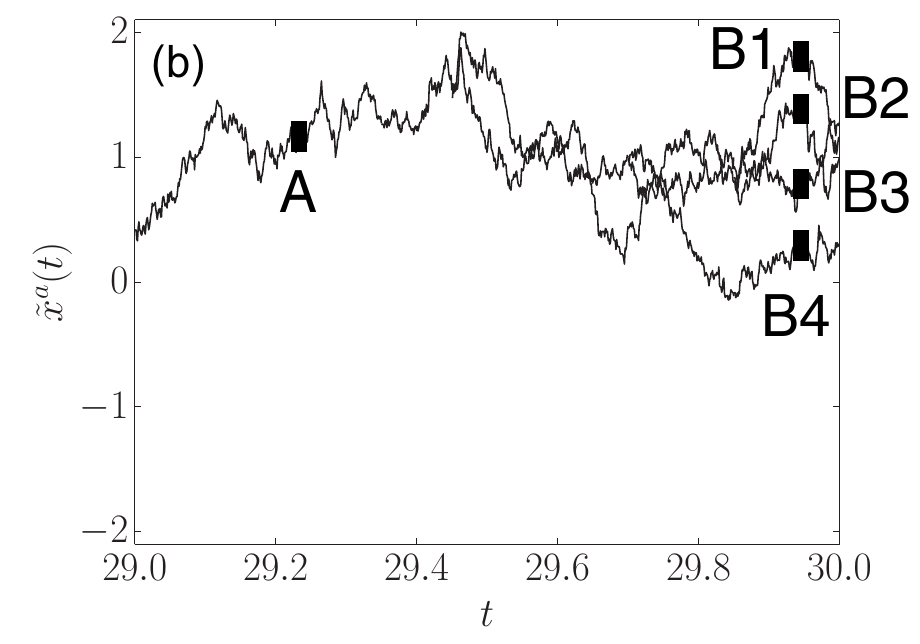
\includegraphics[width=0.42\textwidth]{Nemoto_2016_fig1b.png}
% \caption{$\tiny Z_{\tau}(s) = \left<e^{s \int_0^{\tau} x(t)(1 + x(t)) \, \text{d}t}\right>$. \FigureFrom{nemoto2016population}{1}}
\end{figure}
\vspace{-5pt}
\begin{equation}
\psi(s) = \lim_{\tau \to \infty} \frac{1}{\tau} \log \left<e^{s \int_0^{\tau} x(t)(1 + x(t)) \, \text{d}t}\right>
\end{equation}

\end{frame}

\section{Dynamical phase transitions for active Brownian particles}

\begin{frame}{How does the active work control emerging behaviours?}

\pause
\begin{enumerate}[<+->]
  \item Cloning algoritm $\Rightarrow$ trajectories biased with respect to $\color{CaPink} w_{\tau}$.
  \item Singularities in $\color{green} \psi$.
  \item Description of qualitative changes at dynamical transition.
\end{enumerate}

% \begin{itemize}
%   \item[$\Rightarrow$] Cloning algorithm $\rightarrow$ generate trajectories of systems of ABPs where large deviations of the active work are typical.\pause
%   \begin{itemize}
%     \item[$\rightarrow$] Compute SCGF...
%     \begin{equation}
%       \psi_N(s, \tau) = \frac{1}{\tau} \log\left<e^{- s N \tau w_{\tau}}\right>,
%     \end{equation}
%     \begin{align*}
%       s > 0 \Leftrightarrow \text{large {\bf negative} fluctuations of } w(s)
%     \end{align*}
%     ... biased average of the active work...
%     \begin{equation}
%       w(s) = \left<w_{\tau}\right>_s = - \psi_N^{\prime}(s)/N,
%     \end{equation}
%     ... and rate function.
%     \begin{equation}
%       I_N(w) = \sup_s \left\{- s N w - \psi_N(s)\right\} = - s(w) N w - \psi_N(s(w)).
%     \end{equation}
%     \pause
%     \item[$\rightarrow$] Look for singularities in $I_N/N$ and $\psi_N/N$ $\Rightarrow$ fundamental changes in the mechanisms to produce the associated fluctuations of the active work.
%   \end{itemize}
% \end{itemize}

\end{frame}

\begin{frame}{Unbiased behaviour}

\footfullcitenomark{nemoto2019optimizing}

\insertmovie{0.7}{Nemoto_2019_unbiased.png}{Nemoto_2019_unbiased.mp4}{
% Unbiased trajectory for $\phi = 0.65$, $\tilde{l}_{\rm p} = 40$. \FigureFrom{nemoto2019optimizing}{}
}

% \begin{itemize}
%   \item[$\rightarrow$] Motility-induced phase separation.
% \end{itemize}

\end{frame}

\begin{frame}{Biased behaviours}

\footfullcitenomark{nemoto2019optimizing}

\begin{figure}
\begin{minipage}{0.48\linewidth}
\centering
{\bf CM} ($s < 0$)
\Movie{1}{Nemoto_2019_CM.png}{Nemoto_2019_CM.mp4}
\end{minipage}
\hfill
\begin{minipage}{0.48\linewidth}
\centering
{\bf PSA} ($s > 0$)
\Movie{1}{Nemoto_2019_PSA.png}{Nemoto_2019_PSA.mp4}
\end{minipage}
\hfill\hfill
% \caption{\textit{(Movie)} Biased trajectories for $N = 64$, $\phi = 0.65$, $\tilde{l}_{\rm p} = 40$. {\bf (left)} $s = -3.2$. {\bf (right)} $s = 0.8$. \FigureFrom{nemoto2019optimizing}{}}
\end{figure}

\begin{center}
  CM $\equiv$ collective motion, PSA $\equiv$ phase-separated arrest
\end{center}

\end{frame}

\begin{frame}{Singularities in $\psi$}

\footfullcitenomark{nemoto2019optimizing}

\vspace{-20pt}
\begin{eqnarray}
& \left<w_{\tau}\right>_s = w(s) = - \psi^{\prime}(s)\\
& -w^{\prime}(s) = \psi^{\prime\prime}(s) = \lim_{\tau \to \infty} N \tau \mathrm{Var}(w_{\tau})_s
\end{eqnarray}

\begin{figure}
\centering
\begin{tikzpicture}[scale=1]
\node[anchor=south west,inner sep=0] at (0,0) {
\includegraphics[width=0.60\textwidth]{Nemoto_2019_fig1b.png} };
\draw[->,thick] (5.3,2.7) -- (4.3,1.2) node[left]{$N \nearrow$};
\end{tikzpicture}
\end{figure}

% \begin{itemize}
%   \item[$\rightarrow$] $w$ jumps discontinously to 0 at $s = 0$: PSA.
%   \item[$\rightarrow$] $-w^{\prime} = \psi^{\prime\prime} = \lim_{\tau \to \infty} N \tau \mathrm{Var}(w_{\tau})_s$ jumps discontinously at $s \lesssim 0$: CM.
% \end{itemize}

\end{frame}

\begin{frame}{Polarisation}

\footfullcitenomark{nemoto2019optimizing}

\vspace{-20pt}
\begin{eqnarray}
& \text{polarisation}~ \hat{\nu} =\left|\frac{1}{N} \sum_{i=1}^N \boldsymbol{u}(\theta_i)\right|,~ \bar{\nu}_{\tau} = \frac{1}{\tau} \int_0^{\tau} \hat{\nu}(t) \, \text{d}t\\
& \left<\bar{\nu}_{\tau}\right> = \left<\bar{\nu}_{\tau}\right>_{s=0} = \propto N^{-1/2}
\end{eqnarray}

\begin{figure}
\centering
\begin{tikzpicture}[scale=1]
\node[anchor=south west,inner sep=0] at (0,0) { \includegraphics[width=0.60\textwidth]{Nemoto_2019_fig2a.png} };
\draw[->,thick] (4.3,2.7) node[below right]{$N \nearrow$} -- (4.3,0.8);
\end{tikzpicture}
\end{figure}

\end{frame}

\section{Collective motion mechanism}

\begin{frame}{Characterisation of the CM transition}

\pause
\begin{enumerate}[<+->]
  \item Location $s^*$ of the transition.
    \begin{equation}
    s* \neq 0 \Rightarrow I \neq 0
    \end{equation}
  \item Analytical illustration of collective motion.
  \item Top-down hydrodynamic description.
\end{enumerate}

\end{frame}

\subsection{CM transition point}

\begin{frame}{CM transition point}

\footfullcitenomark{keta2021collective}

\vspace{-25pt}
% \begin{equation}
% \left<\mathcal{A}\right>_s = \frac{\left<\mathcal{A} e^{-s N \tau w_{f, \tau}}\right>_{v_s^{\rm con}}}{\left<e^{-s N \tau w_{f, \tau}}\right>_{v_s^{\rm con}}},~ v_s^{\rm con} = v_0 \left(1 - \frac{2 s D}{v_0^2}\right)
% \end{equation}
\begin{eqnarray}
& w^{\rm free}(s) = 1 - \frac{2 s D}{v_0^2}\\
& s^{\rm con} = s\left(1 - \frac{2 s D}{v_0^2}\right)
\end{eqnarray}

\vspace{-10pt}
\begin{figure}
\centering
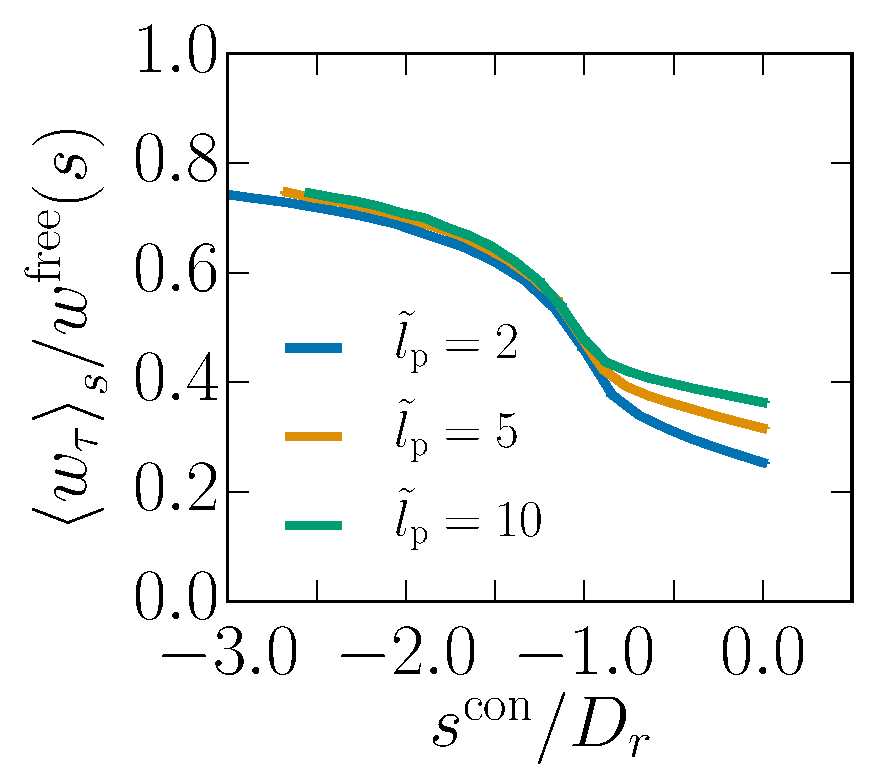
\includegraphics[width=0.45\textwidth]{sWork_Nm5000_Dk6500_To1000-con.eps}
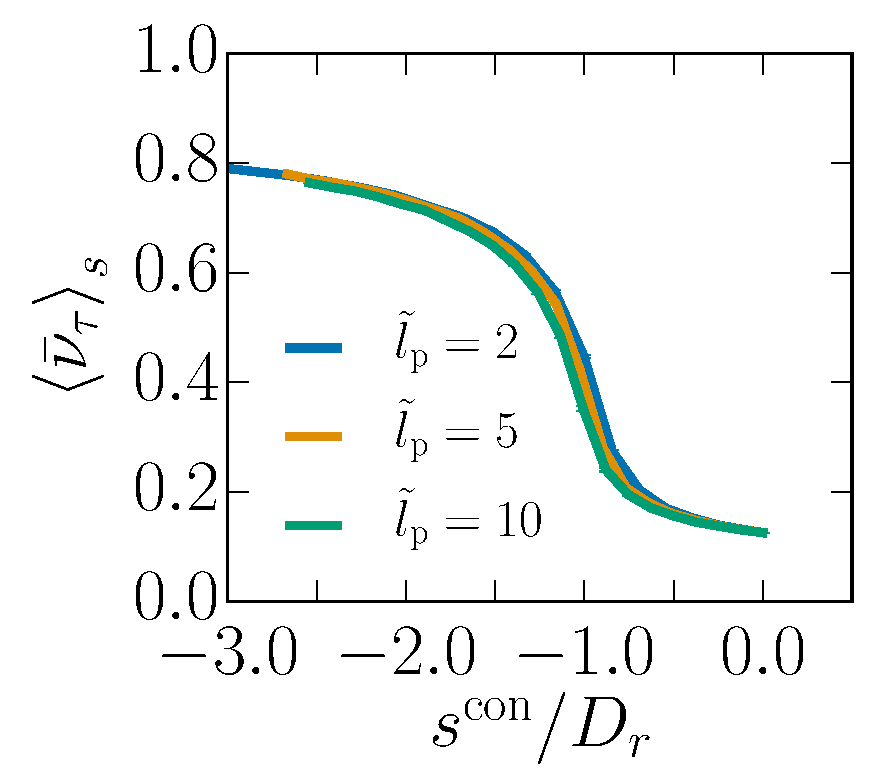
\includegraphics[width=0.45\textwidth]{sOrder_Nm5000_Dk6500_To1000-con.eps}
% \caption{{\bf (left)} Biased average of active work $\left<w_{\tau}\right>_s$. {\bf (right)} Biased average of global order parameter $\left<\bar{\nu}_{\tau}\right>_s$. $N=50$, $\phi = 0.65$.}
\end{figure}

\vspace{-25pt}
\begin{equation}
{s^{\rm con}}^* \approx -D_r
\end{equation}

% \begin{itemize}
%   \item[$\rightarrow$] CM transition at finite $s^* \approx -D_r < 0$.
% \end{itemize}

\end{frame}

\subsection{2 run-and-tumble particles on a ring}

\begin{frame}{Run-and-tumble particles on a ring}

\footfullcitenomark{slowman2016jamming}
\footfullcitenomark{cagnetta2020efficiency}

\begin{figure}
\centering
\includestandalone[width=0.75\textwidth]{rtp}
\end{figure}

\begin{eqnarray}
& \alpha_i \in \{{\color{red} -1}, {\color{green} +1}\}\\
& l = \tau_p(\alpha_i \to -\alpha_i) v_0
\end{eqnarray}

% \begin{itemize}
%   \item[$\rightarrow$] 2 run-and-tumble particles (RTPs).
% \end{itemize}
% \begin{eqnarray}
% \dot{r}_i = \alpha_i v_0 - \partial_{r_i} V(r_{12})
% \end{eqnarray}
% \begin{itemize}
%   \item[$\rightarrow$] $\alpha_i = \pm 1$, tumble ($\alpha_i \to \overline{\alpha}_i = -\alpha_i$) rate $\tau_p^{-1}$, ring length $L$, $V \equiv$ hard core potential.
% \end{itemize}
%
% \pause
% 1 control parameter: $\color{red} L/l$.
% \begin{itemize}
%   \item[$\rightarrow$] persistence length: $l = v_0 \tau_p$.
% \end{itemize}

\end{frame}

\begin{frame}{Active work and biased ensemble}

\vspace{-25pt}
\begin{equation}
\text{active work}~ \dot{w}^{\rm RTP}_f = v_0(\alpha_1 - \alpha_2) \partial_{r_1} V(r_{12})
\end{equation}
% \begin{itemize}
%   \item[$\rightarrow$] $\dot{w}^{\rm RTP}_f = -2 v_0^2$ at contact and 0 otherwise.
% \end{itemize}

\return
\begin{figure}
\centering
\begin{minipage}{0.48\textwidth}
\centering
\includestandalone[width=\textwidth]{rtp}
$\dot{w}^{\rm RTP}_f = 0$
\end{minipage}
\hfill
\begin{minipage}{0.48\textwidth}
\centering
\includestandalone[width=\textwidth]{rtp_contact}
$\dot{w}^{\rm RTP}_f = -2 v_0^2$
\end{minipage}
\end{figure}

\return
\begin{eqnarray}
\text{SCGF}& &\psi^{\rm RTP}(\lambda) = \lim_{\tau \to \infty} \frac{1}{\tau} \log\left<e^{-\lambda \int_0^\tau \dot{w}^{\rm RTP}_f(t) \, \mathrm{d}t}\right>\\
\text{polarisation}& &\nu^{\rm RTP} = \frac{1 + \alpha_1\alpha_2}{2}
% & &P^{\alpha_1\alpha_2}_{\lambda}(r) = \varepsilon_{\lambda}^{\alpha_1\alpha_2}(r) + \gamma_{\lambda}^{\alpha_1\alpha_2,l} \delta(r) + \gamma_{\lambda}^{\alpha_1\alpha_2,r}\delta(L - r)
\end{eqnarray}

\end{frame}

\begin{frame}{Spectral problem}

\footfullcitenomark{touchette2018introduction}
\footfullcitenomark{arnoulx2019active}

\begin{equation}
\psi^{\rm RTP}(\lambda) \boldsymbol{P}_{\lambda} = (\mathcal{L} - \lambda \dot{w}^{\rm RTP}_f) \boldsymbol{P}_{\lambda}
\end{equation}
\return
\begin{equation}
\boldsymbol{P}_{\lambda}(r \equiv r_2 - r_1) \equiv (P^{++}_{\lambda}(r), P^{--}_{\lambda}(r), P^{+-}_{\lambda}(r), P^{-+}_{\lambda}(r))
\end{equation}
\return\pause
\begin{equation}
P^{\alpha_1\alpha_2}_{\lambda}(r) =
\tikzmark{a1}{$\varepsilon^{\alpha_1\alpha_2}_{\lambda}(r)$}
+ \tikzmark{a2}{$\gamma^{\alpha_1\alpha_2,{\rm l}}_{\lambda} \delta(r)$}
+ \tikzmark{a3}{$\gamma^{\alpha_1\alpha_2,{\rm r}}_{\lambda} \delta(L - r)$}
\end{equation}
\return\return

\begin{figure}
\centering
\tikzmark{b1}{\includestandalone[width=0.26\textwidth]{rtp}}
\tikzmark{b2}{\includestandalone[width=0.26\textwidth]{rtp_contact}}
\tikzmark{b3}{\includestandalone[width=0.26\textwidth]{rtp_contact_aligned}}
\end{figure}

\begin{tikzpicture}[remember picture,overlay]
\path[draw=red,thick,->] (a1.south) to[out=-90,in=90] (b1.north);
\path[draw=green,thick,->] (a2.south) to[out=-90,in=90] (b2.north);
\path[draw=blue,thick,->] (a3.south) to[out=-90,in=90] (b3.north);
\end{tikzpicture}

\end{frame}

\begin{frame}{Polarisation averages}

\footfullcitenomark{keta2021collective}

\vspace{-15pt}
\begin{figure}
\centering
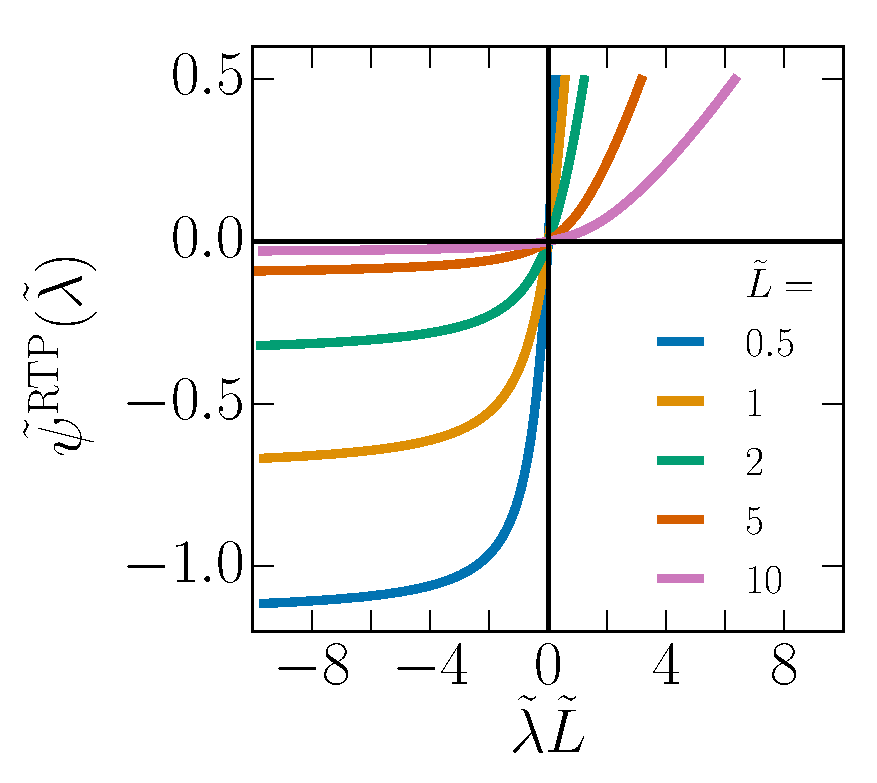
\includegraphics[width=0.35\textwidth]{exactPsiRTP.eps}
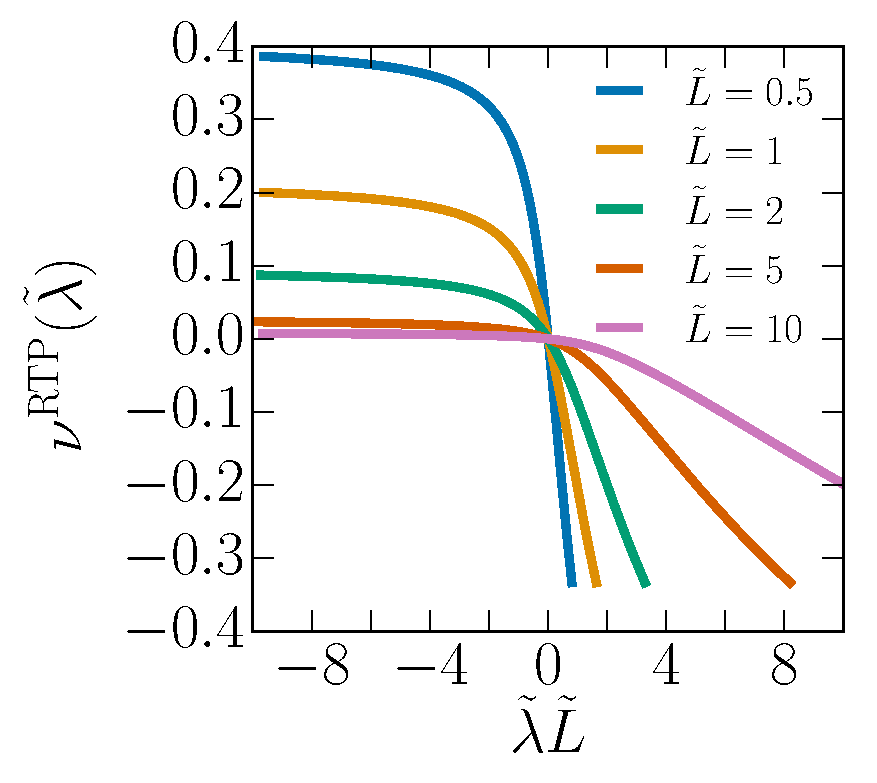
\includegraphics[width=0.35\textwidth]{exactNuRTP.eps}
% \caption{{\bf (left)} Dynamical free energy density. {\bf (right)} Polarisation.}
\end{figure}

\vspace{-10pt}
\begin{equation}
\left<w_f^{\rm RTP}\right>_{\lambda} = -\partial_{\lambda} \psi^{\rm RTP},~ \nu^{\rm RTP} = \frac{1 + \alpha_1\alpha_2}{2}
\end{equation}

\begin{figure}
\centering
\begin{minipage}{0.49\textwidth}
\centering
\includestandalone[width=0.8\textwidth]{rtp_aligned}\\
$\lambda \to -\infty$
\end{minipage}
\begin{minipage}{0.49\textwidth}
\centering
\includestandalone[width=0.8\textwidth]{rtp_contact}\\
$\lambda \to \infty$
\end{minipage}
\end{figure}

% \begin{itemize}
%   \item[$\rightarrow$] Biasing towards positive fluctuations of $w^{\rm RTP}_f$ ($\lambda <0$)
%   \begin{itemize}
%     \item suppresses contact $-\partial_{\lambda} \psi^{\rm RTP} = \left<w^{\rm RTP}_f\right>_{\lambda} \xrightarrow[\lambda \to -\infty]{} 0$,
%     \item favours alignment $\nu^{\rm RTP}(\lambda < 0) > 1/2$.
%   \end{itemize}
% \end{itemize}

\end{frame}

\subsection{Hydrodynamic theory}

\begin{frame}{Top-down fluctuating hydrodynamic description}

\footfullcitenomark{cates2013active}
% \footfullcitenomark{kourbane2018exact}
\footfullcitenomark{cates2019active}

% \vspace{-20pt}
% \begin{itemize}
%   \item[$\rightarrow$] Minimal top-down fluctuating hydrodynamic description for coarse-grained density $\rho(\boldsymbol{r})$ and polarisation $\boldsymbol{P}(\boldsymbol{r})$ fields.
% \end{itemize}
%
% \pause
% \begin{eqnarray}
% &\dot{\rho} = -\nabla \cdot \boldsymbol{J},~ \boldsymbol{J} = \boldsymbol{J}_d + \sqrt{2 \sigma(\rho)} \boldsymbol{\eta}\\
% &\boldsymbol{J}_d = v_0 \rho \boldsymbol{P} - D_c(\rho) \nabla \rho\\
% &\dot{\boldsymbol{P}} = -\gamma(\rho, \boldsymbol{P}) \boldsymbol{f}(\boldsymbol{P}) + b(\rho, \boldsymbol{P}) \nabla \rho + \sqrt{2 \gamma(\rho, \boldsymbol{P})} \boldsymbol{\xi}
% \end{eqnarray}
% \begin{itemize}
%   \item[$\rightarrow$] $\sigma, \gamma \equiv$ noise strengths, $b \equiv$ coupling between polarisation and density gradients, $f \equiv$ force acting on polarisation, $\eta^{\alpha}, \xi^{\alpha} \equiv$ unit-variance zero-mean Gaussian white noises.
% \end{itemize}
%
% \pause
% \begin{equation}
% \text{bias}~ w_{\tau} N \tau = \int_0^{\tau} \int_{[0, L]^2} \omega(\rho, \boldsymbol{P}) \, \mathrm{d}^2\boldsymbol{r} \, \mathrm{d}t
% \end{equation}

\pause
\begin{eqnarray}
\text{continuity}& {\color{red} \dot{\rho}} = - \nabla \cdot {\color{blue} \boldsymbol{J}}\\ \pause
\text{flux}& {\color{blue} \boldsymbol{J}} = {\color{blue} \boldsymbol{J}_d} + \sqrt{2 \sigma({\color{red} \rho})} {\color{yellow} \boldsymbol{\eta}}\\ \pause
& {\color{blue} \boldsymbol{J}_d} = -D_c({\color{red} \rho}) \nabla {\color{red} \rho} \only<5->{+ v_0 {\color{red} \rho} {\color{green} \boldsymbol{P}}}\\ \pause\pause
\text{polarisation}& {\color{green} \dot{\boldsymbol{P}}} = -\gamma({\color{red} \rho}, {\color{green} \boldsymbol{P}}) \boldsymbol{f}({\color{green} \boldsymbol{P}}) \only<7->{+ b({\color{red} \rho}, {\color{green} \boldsymbol{P}}) \nabla {\color{red} \rho} \only<8->{+ \sqrt{2 \gamma({\color{red} \rho}, {\color{green} \boldsymbol{P}})} {\color{yellow} \boldsymbol{\xi}}}}
\end{eqnarray}
\pause\pause\pause

\return
\begin{equation}
\text{bias}~ {\color{CaPink} w_{\tau}} N \tau = \int_0^{\tau} \int_{[0, L]^2} {\color{CaPink} \omega}({\color{red} \rho}, {\color{green} \boldsymbol{P}}) \, \mathrm{d}^2\boldsymbol{r} \, \mathrm{d}t
\end{equation}

\end{frame}

\begin{frame}{Probability of trajectories}

\footfullcitenomark{bertini2015macroscopic}

\vspace{-20pt}
\begin{eqnarray}
& {\color{red} \dot{\rho}} = -\nabla \cdot \left({\color{blue} \boldsymbol{J}_d} + \sqrt{2 \sigma({\color{red} \rho})} {\color{yellow} \boldsymbol{\eta}}\right)\\
& {\color{green} \dot{\boldsymbol{P}}} = -\gamma({\color{red} \rho}, {\color{green} \boldsymbol{P}}) \boldsymbol{f}({\color{green} \boldsymbol{P}}) + b({\color{red} \rho}, {\color{green} \boldsymbol{P}}) \nabla {\color{red} \rho} + \sqrt{2 \gamma({\color{red} \rho}, {\color{green} \boldsymbol{P}})} {\color{yellow} \boldsymbol{\xi}}\\
& {\color{CaPink} w_{\tau}} N \tau = \int_0^{\tau} \int_{[0, L]^2} {\color{CaPink} \omega}({\color{red} \rho}, {\color{green} \boldsymbol{P}}) \, \mathrm{d}^2\boldsymbol{r} \, \mathrm{d}t
\end{eqnarray}

\pause
\return
\begin{center}
  \bf hydrodynamic variables
\end{center}
\begin{eqnarray}
& \boldsymbol{r} \to \boldsymbol{r}/L,~ t \to D t/L^2
\end{eqnarray}

\pause
\begin{eqnarray}
& P[{\color{red} \rho}, {\color{blue} \boldsymbol{J}}, {\color{green} \boldsymbol{P}}] \propto \exp\left(-L^2 \int_0^{\tau} \int_{[0, 1]^2} S({\color{red} \rho}, {\color{blue} \boldsymbol{J}}, {\color{green} \boldsymbol{P}}) \, \mathrm{d}^2\boldsymbol{r} \, \mathrm{d}t\right)\\ \pause
& S = \frac{D}{4 \sigma}\left|{\color{blue} \boldsymbol{J}} - {\color{blue} \boldsymbol{J}_d}\right|^2 + \frac{1}{4 D \gamma} \left|\frac{D}{L} {\color{green} \dot{\boldsymbol{P}}} + \gamma \boldsymbol{f} L - b\nabla {\color{red} \rho}\right|^2 + \frac{s L^2}{D} {\color{CaPink} \omega}
\end{eqnarray}

% \begin{itemize}
%   \item[$\rightarrow$] Hydrodynamic variables.
% \end{itemize}
%
% \begin{eqnarray}
% &\tilde{\boldsymbol{r}} = \boldsymbol{r}/L,~ \tilde{t} = D t / L^2\\
% &\tilde{\rho}(\tilde{\boldsymbol{r}}, \tilde{t}) = \rho(\tilde{\boldsymbol{r}} L, \tilde{t} L^2/D),~ \tilde{\boldsymbol{P}}(\tilde{\boldsymbol{r}}, \tilde{t}) = \boldsymbol{P}(\tilde{\boldsymbol{r}} L, \tilde{t} L^2 D)
% \end{eqnarray}
%
% \pause
% \return
% \begin{itemize}
%   \item[$\rightarrow$] Probability of observing a trajectory in the biased ensemble.
% \end{itemize}
%
% \begin{eqnarray}
% &P[\tilde{\rho}, \tilde{\boldsymbol{J}}, \tilde{\boldsymbol{P}}] \propto \exp\left(-L^2 \int_0^{\tilde{\tau}} \int_{[0, 1]^2} S(\tilde{\rho}, \tilde{\boldsymbol{J}}, \tilde{\boldsymbol{P}}) \, \mathrm{d}^2\tilde{\boldsymbol{r}} \, \mathrm{d}\tilde{t}\right)\\
% &S = \frac{D}{4 \sigma}|\tilde{\boldsymbol{J}} - \tilde{\boldsymbol{J}}_d|^2 + \frac{1}{4 D \gamma}\left|\frac{D}{L} \dot{\tilde{\boldsymbol{P}}} + \gamma \boldsymbol{f} L - b \nabla \tilde{\rho}\right|^2 + \frac{s L^2}{D} \omega
% \end{eqnarray}

\end{frame}

\begin{frame}{Mean-field analysis}

\footfullcitenomark{keta2021collective}

\begin{equation}
S = \only<1-7>{\only<1-5>{\only<1-3>{\frac{D}{4 \sigma}}\only<1-2>{\left|{\color{blue} \boldsymbol{J}} - {\color{blue} \boldsymbol{J}_d}\right|^2}\only<3>{\cancel{\left|{\color{blue} \boldsymbol{J}} - {\color{blue} \boldsymbol{J}_d}\right|^2}} \only<1-3>{+} \frac{1}{4 D \gamma} \left|\only<1>{\frac{D}{L} {\color{green} \dot{\boldsymbol{P}}}}\only<2>{\cancel{\frac{D}{L} {\color{green} \dot{\boldsymbol{P}}}}} \only<1-2>{+} \gamma \boldsymbol{f} L \only<1>{- b\nabla {\color{red} \rho}}\only<2>{\cancel{- b\nabla {\color{red} \rho}}}\right|^2}\only<6->{\frac{{\color{red} \bar{\rho}} L^2}{D} \mathcal{J}({\color{green} \boldsymbol{P}})} + \frac{s L^2}{D} {\color{CaPink} \omega}}\only<8->{\frac{{\color{red} \bar{\rho}} L^2}{D} \left[s \left<{\color{CaPink} w_{\tau}}\right> + \frac{1}{2}(D_r + s c_{\color{CaPink} \omega})|{\color{green} \boldsymbol{P}}|^2 + \mathcal{O}(|{\color{green} \boldsymbol{P}}|^4)\right]}
\end{equation}

\pause
\return
\begin{center}
$({\color{red} \rho}, {\color{blue} \boldsymbol{J}}, {\color{green} \boldsymbol{P}})$ independent of space and time
\end{center}
\pause\pause\pause

\return
\begin{equation}
\text{LDP on polarisation}~ P_{s=0}[{\color{red} \bar{\rho}}, {\color{blue} \boldsymbol{J}_d}, {\color{green} \boldsymbol{P}}] \propto \exp\left(-\frac{L^2 t}{D} {\color{red} \bar{\rho}} \mathcal{J}({\color{green} \boldsymbol{P}})\right)
\end{equation}
\pause

\pause
\return
\begin{eqnarray}
\text{analytical derivation}& & \mathcal{J}({\color{green} \boldsymbol{P}}) = \frac{1}{2} D_r |{\color{green} \boldsymbol{P}}|^2 + \mathcal{O}(|{\color{green} \boldsymbol{P}}|^4)\\
\text{Taylor expansion}& &{\color{CaPink} \omega}({\color{red} \bar{\rho}}, {\color{green} \boldsymbol{P}}) = {\color{red} \bar{\rho}} \left[\left<{\color{CaPink} w_{\tau}}\right> + \frac{c_{\color{CaPink} \omega}}{2} |{\color{green} \boldsymbol{P}}|^2 + \mathcal{O}(|{\color{green} \boldsymbol{P}}|^4)\right]
\end{eqnarray}
\pause

% \begin{itemize}
%   \item[$\rightarrow$] $(\tilde{\rho}, \tilde{\boldsymbol{J}}, \tilde{\boldsymbol{P}})$ independent of space and time \pause $\Rightarrow$ the action $S$ is minimised for $\tilde{\boldsymbol{J}} = \tilde{\boldsymbol{J}}_d$
%   \begin{equation}
%   S = \frac{\bar{\rho} L^2}{D} \left[s \left<w_{\tau}\right> + \frac{1}{2} |\boldsymbol{P}|^2 (D_r + s c_{\omega}) + \mathcal{O}(|\boldsymbol{P}|^4)\right]
%   \end{equation}
%   from the properties of the ABP system.
% \end{itemize}
%
% \pause
% \begin{figure}
% \centering
% 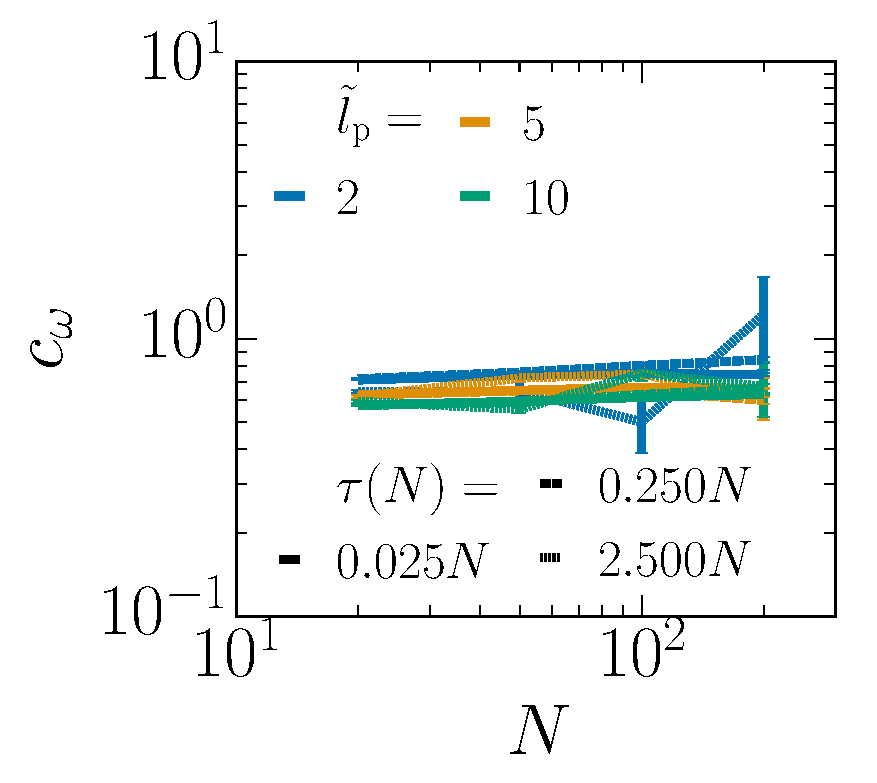
\includegraphics[width=0.3\textwidth]{covPW_Dk6500.eps}
% \caption{Covariance parameter $c_{\omega} = \frac{\bar{\rho} \tau^2 L^4 D_r^2}{2} \mathrm{Cov}(w_{\tau}, |\boldsymbol{\nu}_{\tau}|^2)$.}
% \end{figure}
%
% \begin{itemize}
%   \item[$\rightarrow$] $c_{\omega}$ constant $\Rightarrow$ spontaneous symmetry breaking for $s < -D_r/c_{\omega}$.
% \end{itemize}

\end{frame}

\begin{frame}[t]{Spontaneous symmetry breaking}

\footfullcitenomark{goldenfeld2018lectures}
\footfullcitenomark{keta2021collective}

\vspace{-25pt}
\begin{equation}
S = \frac{{\color{red} \bar{\rho}} L^2}{D} \left[s \left<{\color{CaPink} w_{\tau}}\right> + \frac{1}{2}(D_r + s c_{\color{CaPink} \omega})|{\color{green} \boldsymbol{P}}|^2 + \mathcal{O}(|{\color{green} \boldsymbol{P}}|^4)\right]
\end{equation}
\pause
\only<2-3>{
\return
\begin{center}
analogy with a \textbf{ferromagnet}
\end{center}
\begin{equation}
\mathcal{L}(H = 0) = a(T_c) (T - T_c) {\color{green} \eta}^2 + \mathcal{O}({\color{green} \eta}^4),~ T_c \propto J
\end{equation}
\pause
\begin{figure}
\centering
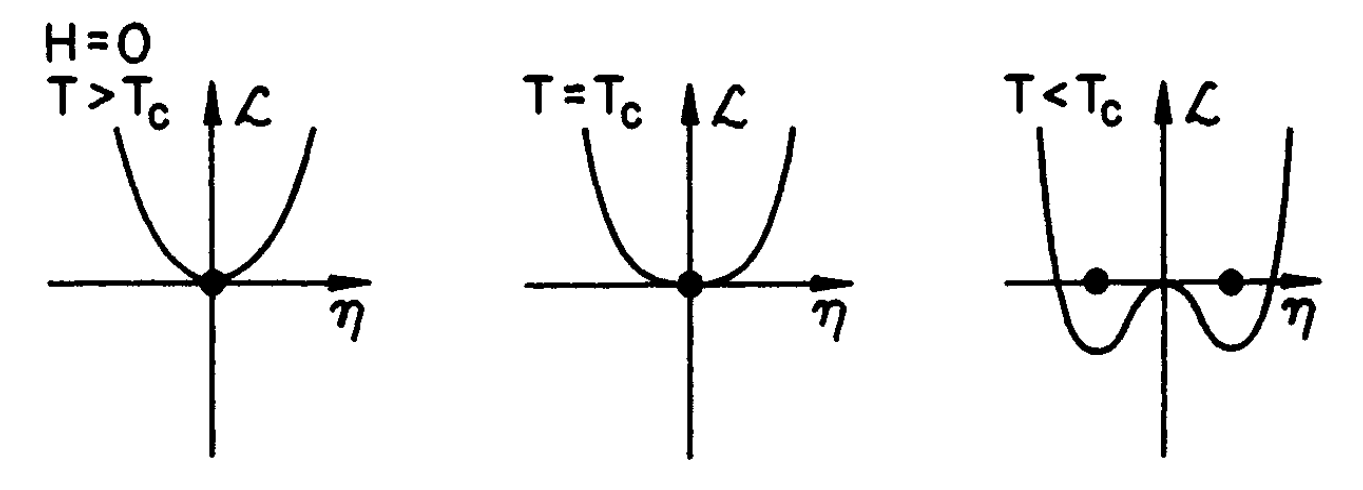
\includegraphics[width=0.80\textwidth]{Goldenfeld_1992_fig5.1.png}
\end{figure}
}
\only<4->{
\begin{figure}
\includestandalone[width=0.5\textwidth]{action}
\end{figure}
}

\end{frame}

\section{Conclusion}

\begin{frame}{Conclusion}

\pause
\begin{itemize}[<+->]
  \item We have introduced a model of {\bf active Brownian particles} biased with respect to a measure of the {\bf averaged dissipated power} (active work $w_{\tau}$).
  \item This model of isotropic active matter displays {\bf phase-separated arrest} (PSA) when $w_{\tau}$ is decreased ($s > 0$) and {\bf collective motion} (CM) when $w_{\tau}$ is increased ($s < 0$).
  \item This transition to CM happens at {\bf finite biasing} $s^* \sim -D_r$ implying that these fluctuations are very distinct from the unbiased behaviour.
  \item We have computed particle alignment exactly for a system of 2 particles, and showed that increased $w_{\tau}$ is accompanied by {\bf effective aligning interactions}.
  \item We have proposed a {\bf fluctuating hydrodynamic theory} which captures the emergence of polar order in the biased state.
\end{itemize}

\end{frame}

%% THANK YOU

{
\footerwithoutframenumber
\begin{frame}[noframenumbering]

\begin{center}
\Huge
Thank you!
\end{center}

\end{frame}
}

%% SUPPLEMENTAL FRAMES

{
\footerwithoutframenumber

\begin{frame}[noframenumbering]{Temporal boundary conditions}

\footfullcitenomark{nemoto2016population}

\vspace{-12pt}
\begin{itemize}
  \item[$\rightarrow$] In the $s$-ensemble of trajectories $x(0 \leq t \leq \tau)$, $t=0$ and $t=\tau$ are boundaries $\Rightarrow$ dynamical analogue of boundary effects.
\end{itemize}

\begin{figure}
\centering
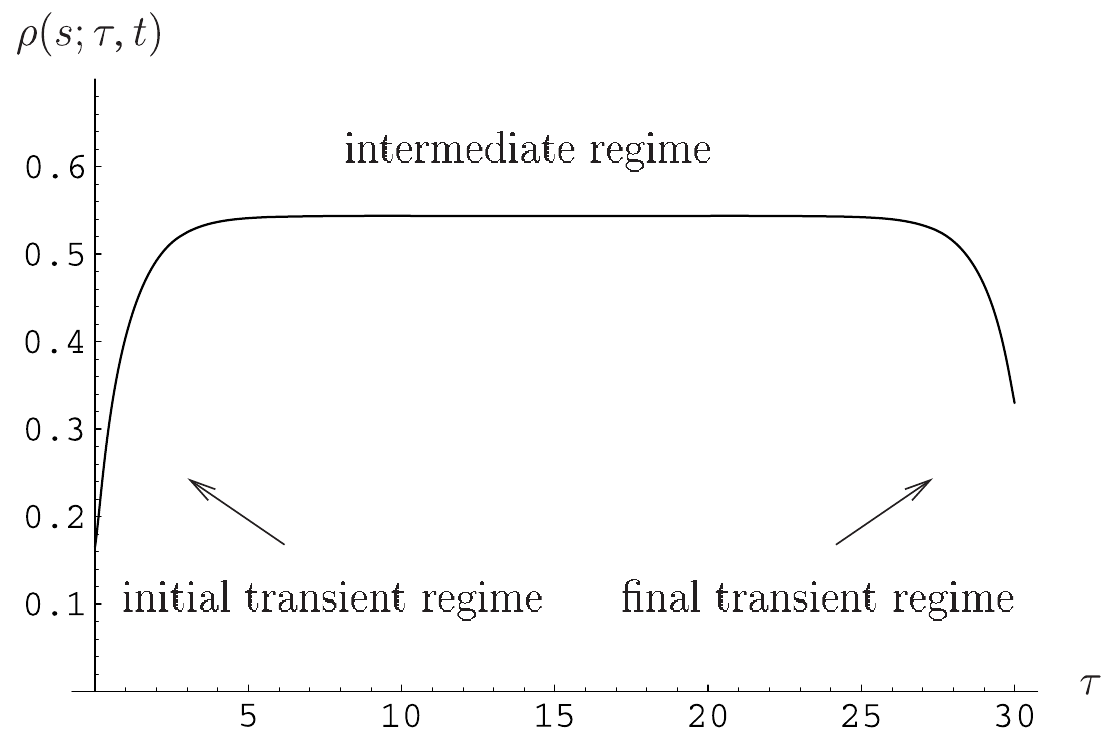
\includegraphics[width=0.40\textwidth]{Garrahan_2009_fig7.png}
\caption{\FigureFrom{garrahan2009first}{7}}
\end{figure}

\vspace{-25pt}
\begin{eqnarray}
&P_{\rm end}(x) = \lim_{\tau \to \infty} \left<\delta(x(\tau) - x)\right>_s\\
&P_{\rm ave}(x) = \lim_{\tau \to \infty} \left<\tau^{-1} \int_0^{\tau} \delta(x(t) - x) \mathrm{d}t\right>_s
\end{eqnarray}

\end{frame}

\begin{frame}[noframenumbering]{Spectral problem}

\footfullcitenomark{touchette2018introduction}

\vspace{-25pt}
\begin{eqnarray}
\text{SDE}& &\dot{\boldsymbol{X}} = F(\boldsymbol{X}) + \sqrt{2 D} \boldsymbol{\eta}\\
\text{Fokker-Planck equation}& &\frac{\partial}{\partial t} P(\boldsymbol{x}, t) = \mathcal{L} P(\boldsymbol{x}, t)\\
& &P(\boldsymbol{x}, t) = P(\boldsymbol{X}(t) = \boldsymbol{x})\\
\text{observable}& &A_{\tau} = \frac{1}{\tau} \int_0^{\tau} f(\boldsymbol{X}(t)) \, \mathrm{d}t\\
\text{SCGF}& &\psi(s) = \lim_{\tau \to \infty} \frac{1}{\tau} \log\left<\exp(-s \tau A_{\tau})\right>
\end{eqnarray}

\return
\begin{itemize}
  \item[$\rightarrow$] $\psi(s)$ is the largest eigenvalue of $\mathcal{L} - s f$.
\end{itemize}

\begin{eqnarray}
&\lambda(s) l(\boldsymbol{x}) = (\mathcal{L} - s f(\boldsymbol{x})) l(\boldsymbol{x})\\
&P_{\rm end}(\boldsymbol{x}) = l(\boldsymbol{x})\\
&\lambda(s) r(\boldsymbol{x}) = (\mathcal{L}^{\dagger} - s f(\boldsymbol{x})) r(\boldsymbol{x})\\
&P_{\rm ave}(\boldsymbol{x}) = l(\boldsymbol{x}) r(\boldsymbol{x})
\end{eqnarray}

\end{frame}

\begin{frame}[noframenumbering]{Interest of bounds}

\footfullcitenomark{jack2020ergodicity}

\begin{center}
``Large deviations occur according to the least unlikely mechanism.''
\end{center}

% \pause
\return
\begin{equation}
{\color{red} I_A}(w) \leq I(w) \leq {\color{blue} I_B}(w) \text{ the closer the better}
\end{equation}

\end{frame}

\begin{frame}[noframenumbering]{Modified dynamics}

\begin{eqnarray}
&\dot{\boldsymbol{r}}_i = {\color{red} v_s^{\rm con}} \boldsymbol{u}(\theta_i) - D \nabla_i U + \sqrt{2 D} \boldsymbol{\eta}_i\\
&\dot{\theta}_i = {\color{red}- D_r \frac{\partial}{\partial \theta_i} U^{\rm con}_g} + \sqrt{2 D_r} \xi_i
\end{eqnarray}

% \pause
% \begin{itemize}
%   \item[$\Rightarrow$] Upper bound to the rate function.
% \end{itemize}

\begin{eqnarray}
&I(w) \leq \lim_{\tau \to \infty} \mathcal{D}_{\rm KL}(P^{\rm mod}_{g(w)} || P)\\
&\mathcal{D}_{\rm KL}(P^{\rm mod}_{g(w)} || P) = \left<\log P^{\rm mod}_{g(w)} / P\right>_{\rm mod} = f[\{\theta_i(t)\}, g(w)]
\end{eqnarray}

\end{frame}

\begin{frame}[noframenumbering]{Contraction principle}

% \begin{itemize}
%   \item[$\rightarrow$] Since probabilities are measured on the exponential scale, the probability of any large fluctuation should be approximated by the probability of the least improbable event leading to this fluctuation.
% \end{itemize}
\begin{equation}
I_{h(A)}(b) = \inf_{a:h(a)=b} I_A(a)
\end{equation}

% \pause
% \return
% \begin{itemize}
%   \item[$\Rightarrow$] Lower bound to the rate function.
% \end{itemize}

% \begin{eqnarray}
% \text{polarisation rate function}& &J(\nu)\\
% \text{joint rate function}& &I_2(w, \nu)
% \end{eqnarray}

% \begin{equation}
% {\color{blue} I(w)} \only<2->{{\color{red} \underset{\rm CP}{=}} \inf_{\nu} I_2(w, \nu) \only<3->{= I_2(w, \nu(w)) \only<4->{{\color{blue}\geq} \inf_{w^{\prime}} I_2(w^{\prime}, \nu(w)) {\color{red} \only<5->{\underset{\rm CP}{=} {\color{blue} \mathcal{J}_1(\nu(w))}}}}}}
% \end{equation}
\return
\begin{equation}
{\color{blue} I(w)} {\color{red} \underset{\rm CP}{=}} \inf_{\nu} I_2(w, \nu) = I_2(w, \nu(w)) {\color{blue}\geq} \inf_{w^{\prime}} I_2(w^{\prime}, \nu(w)) {\color{red} \underset{\rm CP}{=}} {\color{blue} \mathcal{J}_1(\nu(w))}
\end{equation}
% \pause\pause\pause

\end{frame}

\begin{frame}[noframenumbering]{Bounds to the rate function}

\begin{figure}
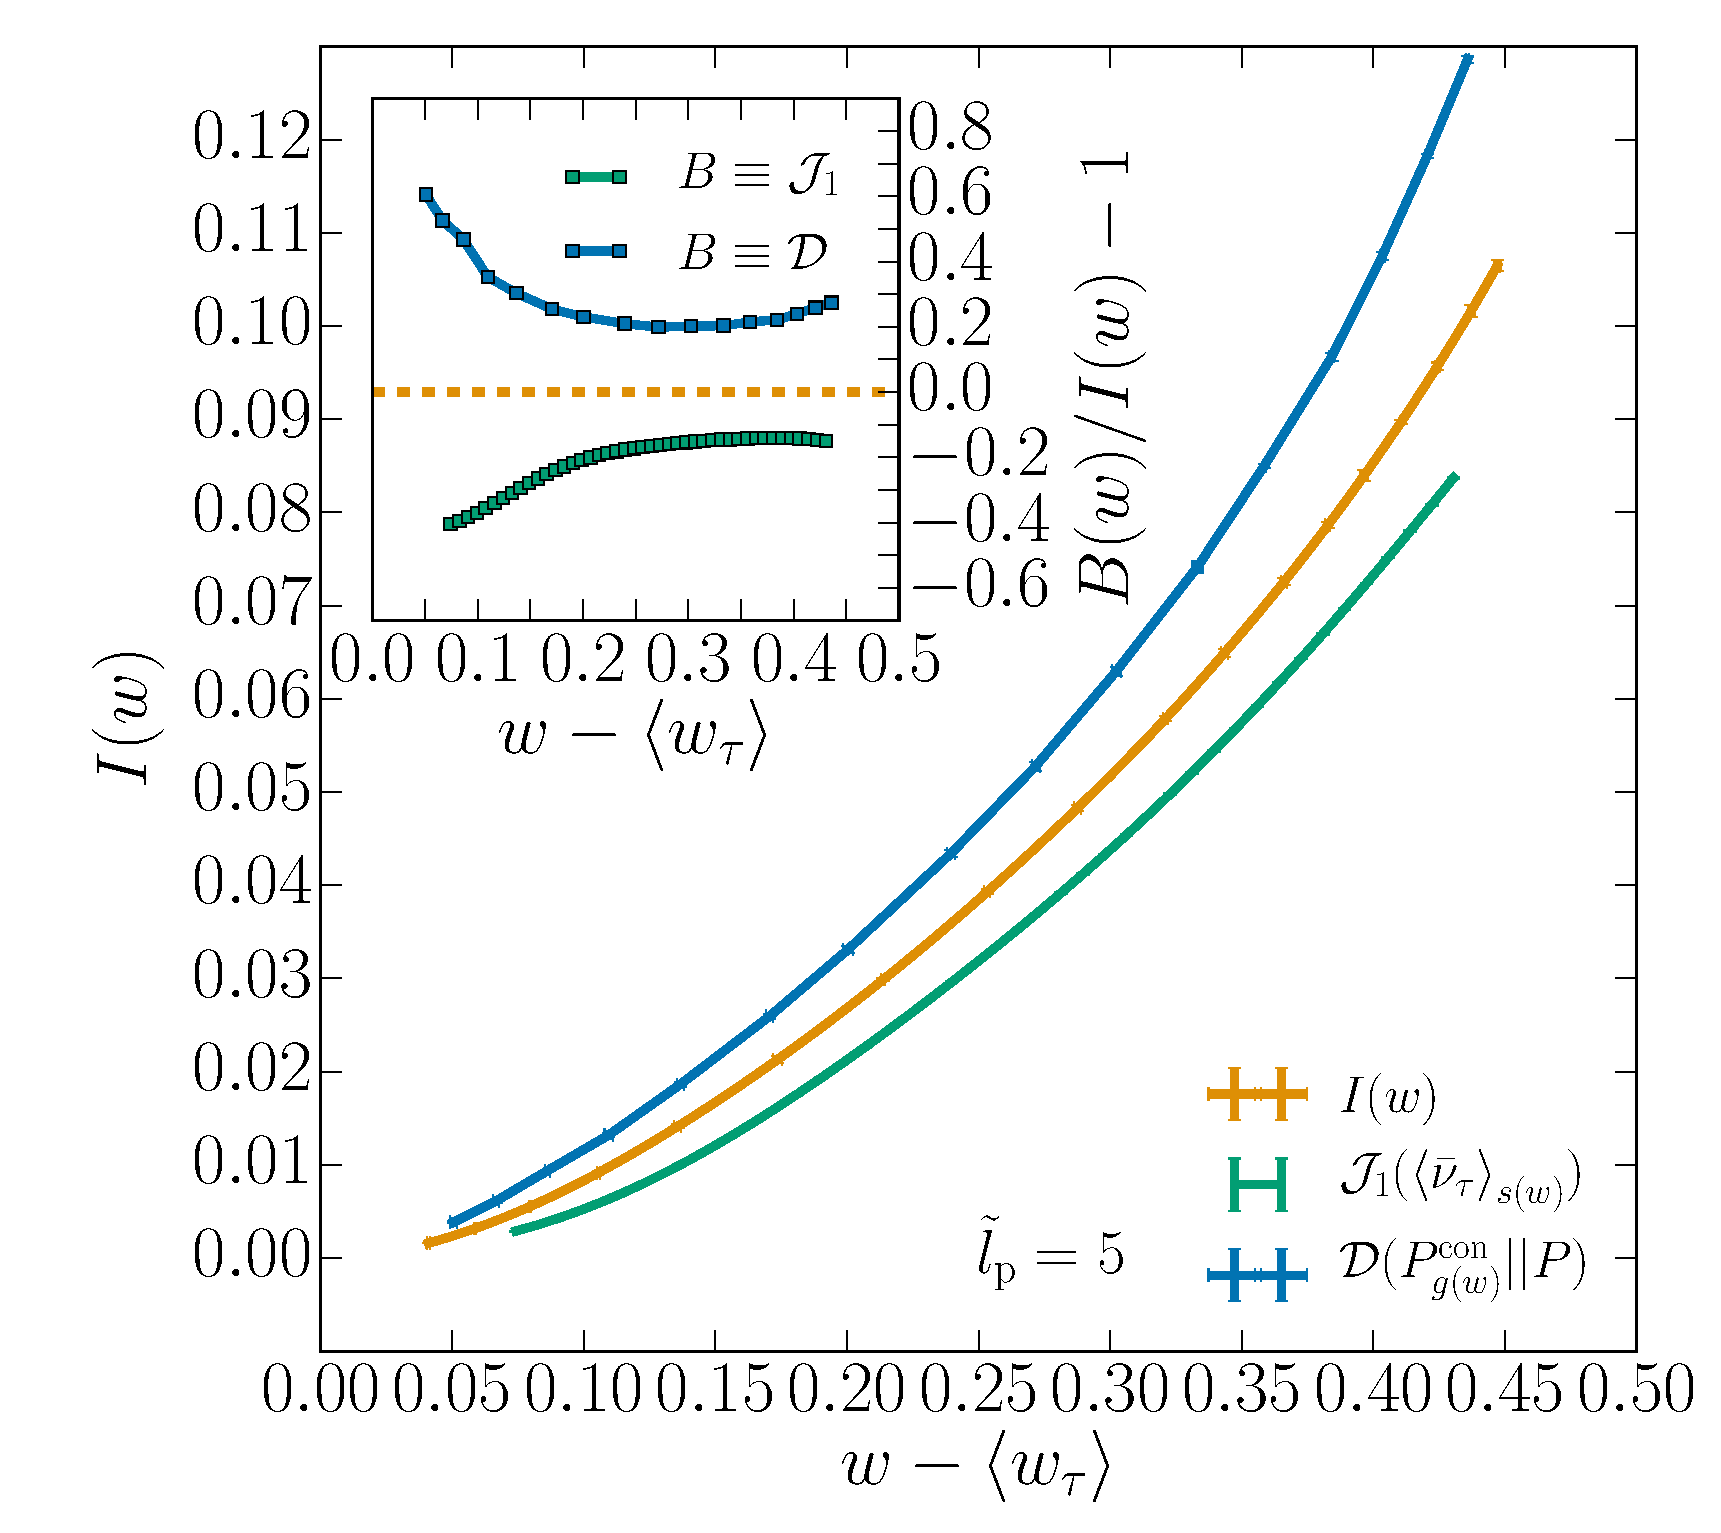
\includegraphics[width=0.45\textwidth]{boundRate.eps}
\includegraphics[width=0.45\textwidth]{boundRate40.eps}
% \caption{Bounds to the rate function $I(w)$.}
\end{figure}

% \begin{itemize}
%   \item[$\rightarrow$] In the CM state ($w \geq w^*$) both bounds perform well $\Rightarrow$ fluctuations of $w_{\tau}$ are strongly coupled to those of $\bar{\nu}_{\tau}$.
% \end{itemize}

\end{frame}

\begin{frame}[noframenumbering]{Hydrodynamic active work}

\begin{eqnarray}
& \omega(\bar{\rho}, \boldsymbol{P}) = \left<\bar{\rho} w_{\tau}\right>_{\boldsymbol{h}(\boldsymbol{P})} = \frac{\left<\bar{\rho} w_{\tau} \exp(-\tau N \boldsymbol{h}(\boldsymbol{P}) \cdot \bar{\boldsymbol{\nu}}_{\tau})\right>}{\left<\exp(-\tau N \boldsymbol{h}(\boldsymbol{P}) \cdot \bar{\boldsymbol{\nu}}_{\tau})\right>}\\
& \bar{\boldsymbol{\nu}}_{\tau} = \frac{1}{\tau} \int_0^{\tau} \frac{1}{N} \sum_{i=1}^N \boldsymbol{u}(\theta_i(t)) \, \mathrm{d}t,~ \left<\bar{\boldsymbol{\nu}}_{\tau}\right>_{\boldsymbol{h}(\boldsymbol{P})} = \boldsymbol{P}\\
& \omega(\bar{\rho}, \boldsymbol{P}) = \bar{\rho}\left[\left<w_{\tau}\right> + \frac{c_{\omega}}{2} |\boldsymbol{P}|^2 + \mathcal{O}(|\boldsymbol{P}|^4)\right]\\
& c_{\omega} = \frac{\bar{\rho} \tau^2 L^4 D_r^2}{2} \mathrm{Cov}(w_{\tau}, |\bar{\boldsymbol{\nu}}_{\tau}|^2)
\end{eqnarray}

\begin{figure}
\centering
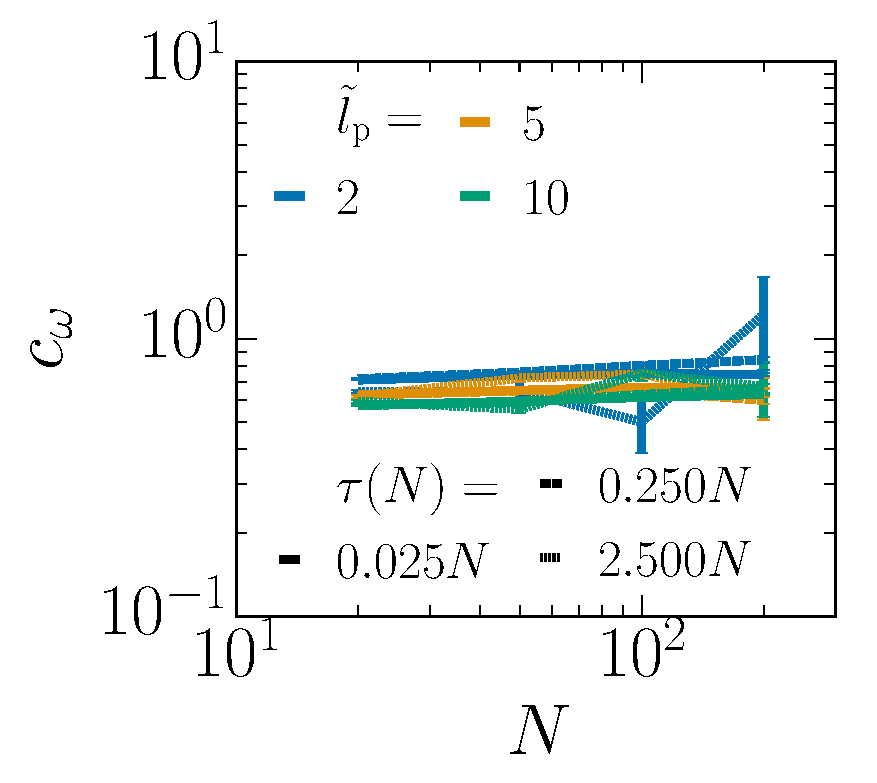
\includegraphics[width=0.3\textwidth]{covPW_Dk6500.eps}
% \caption{Covariance parameter $c_{\omega} = \frac{\bar{\rho} \tau^2 L^4 D_r^2}{2} \mathrm{Cov}(w_{\tau}, |\boldsymbol{\nu}_{\tau}|^2)$.}
\end{figure}

\end{frame}

\begin{frame}[noframenumbering]{Suppression of density fluctuations}

\footfullcitenomark{dolezal2019large}

\vspace{-15pt}
\begin{itemize}
  \item At $\boldsymbol{P} = 0$, biasing w.r.t. $w_{\tau}$ is equivalent to biasing w.r.t. $|\tilde{\rho}_{\boldsymbol{q}}|^2$.
\end{itemize}

\begin{equation}
S_s(\boldsymbol{q}) = \left<|\tilde{\rho}_{\boldsymbol{q}}|^2\right>_s = \begin{cases} \chi_0, &s = 0 \\ b_s q, &s < 0 \end{cases}
\end{equation}
\begin{itemize}
  \item[$\Rightarrow$] We expect hyperuniformity in the isotropic $s < 0$ phase for $N \gg 1$.
\end{itemize}

\begin{figure}
\centering
\includegraphics[width=0.5\textwidth]{S_Nn1000_Dk6500_Ll5000_NCo1000.eps}
\caption{Biased structure factor $S_s$.}
\end{figure}

\vspace{-10pt}
\begin{itemize}
  \item[$\rightarrow$] Finite system shows suppression of density fluctuations for $s < 0$.
\end{itemize}

\end{frame}

}

\end{document}
